%! TEX root = ../main.tex
% ==============================================================
% IMMUTABLE — generated automatically, do not edit this block
%
% — Provenance ───────────────────────────────────────────────────
%   script            : plotter.py
%   computed_in       : 
%   plot_type         : wave_stability
%   data_class        : 
%   generated_at      : 2026-04-24T15:40:40
%   findings_doc      : 
%
% — Thesis context ──────────────────────────────────────────────
%   chapter           : 04
%   caption_label     : fig:ch04_wave_stability
%   caption_short     : Wave-train stability (autocorrelation at lag-1-period) versus wave frequency for 4 probes, 293 wave runs
%
% — Filters ────────────────────────────────────────────────────
%   panel             : full
%   wind              : 
%   amplitude [V]     : 
%   frequency [Hz]    : 0.9, 1.6
%   probes            : 9373/170, 12400/250, 9373/340, 8804/250
%   run_category      : 
%   quality_flag      : 
%   mooring           : 
%
% — Data provenance ────────────────────────────────────────────
%   n_runs            : 637
%   in_probes_used    : 9373/170+9373/340, 9373/250
%   out_probes_used   : 11800/250, 12400/170+12400/340, 12400/250
%   probe_configs     : initial_setup, march2026_better_rearranging, march2026_rearranging, nov_normalt_oppsett
%   non_final_config_n: 169
%   datasets        :
%     PROCESSED-20260326-ProbePos4_31_FPV_2-tett6roof-under9Mooring-height100-lowrange
%     PROCESSED-20260327-ProbePos4_31_FPV_2-tett6roof-under9Mooring30-height100-lowrange
%   run_paths       :
%     (omitted — aggregate over > threshold runs, see datasets)
%
% — Method / numerical parameters ─────────────────────────────
%   grouper           : 
%   collapse_panels   : 
%   fft_window_hz     : 
%   extra_params      : 
%
% — Summary stats cited in caption ────────────────────────────
%   (none registered — pass extra_stats=... to build_fig_meta)
%
% — Subfigures available ───────────────────────────────────────
%     FIGURES/ch04_wave_stability.pdf
% ── end immutable block ─────────────────────────────────────────
\begin{figure}[htbp]
  \centering
  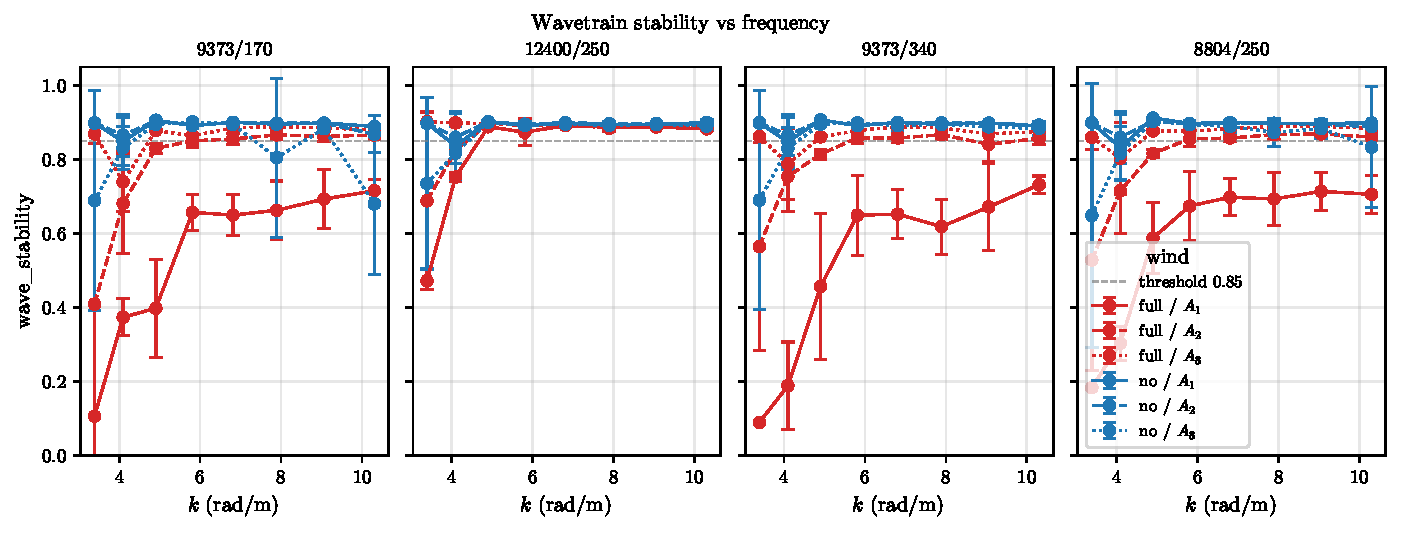
\includegraphics[width=\linewidth]{FIGURES/ch04_wave_stability.pdf}
  \caption[Wave-train stability (autocorrelation at lag-1-period) versus wave frequency for 4 probes, 293 wave runs]{
    Wave-train stability (autocorrelation at lag-1-period) versus wave frequency for 4 probes, 293 wave runs. Colour = wind condition; linestyle = wave amplitude. Error bars: standard deviation across repeated runs at the same (frequency, amplitude). Dashed line: quality threshold 0.85 — runs below this are dominated by wind-wave noise at the IN probe.
  }
  \label{fig:ch04_wave_stability}
\end{figure}
